\section{Memory Layout}

\frame{\tableofcontents[currentsubsection]}

\begin{frame}
    \frametitle{Arrays}
    \begin{center}
        \begin{tikzpicture}
            \draw[help lines] (-2,0) grid (8,1);
            \draw[thick] (0,0) grid (6,1);
            \foreach \x in {0,...,5} {
                \node[font=\tiny] at ($ (\x,0.5) + (0.5,0) $) { \texttt{xs[\x]} };
            }
        \end{tikzpicture}
    \end{center}
    \vskip4mm
    \begin{itemize}
        \item One piece of contiguous memory
    \end{itemize}
\end{frame}

\begin{frame}
    \frametitle{Arrays}
    \code[language=c++14]{array.cpp}
\end{frame}

\begin{frame}
    \frametitle{Linked Lists}
    \begin{center}
        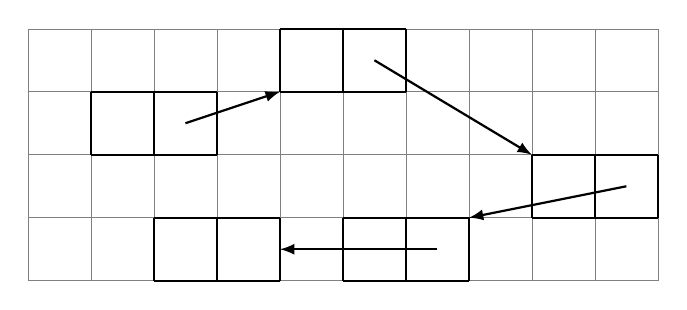
\begin{tikzpicture}[link/.style={thick,-latex},scale=0.8,transform shape]
            \draw[help lines] (0,0) grid (10,4);
            \draw[thick] (1,2) grid ++(2,1);
            \draw[thick] (4,3) grid ++(2,1);
            \draw[thick] (5,0) grid ++(2,1);
            \draw[thick] (2,0) grid ++(2,1);
            \draw[thick] (8,1) grid ++(2,1);

            \draw[link] (2.5,2.5) -- (4,3);
            \draw[link] (5.5,3.5) -- (8,2);
            \draw[link] (9.5,1.5) -- (7,1);
            \draw[link] (6.5,0.5) -- (4,0.5);
        \end{tikzpicture}
    \end{center}
    \vskip4mm
    \begin{itemize}
        \item List consists of series of nodes
        \item Each node has two fields
              \begin{itemize}
                \item Item
                \item Reference to next node
              \end{itemize}
        \item Nodes spread across memory
    \end{itemize}
\end{frame}

\begin{frame}
    \frametitle{Linked Lists in Code}
    \code[language=csharp]{LinkedList.cs}
\end{frame}

\begin{frame}
    \frametitle{Creating a Linked List}
    \begin{center}
        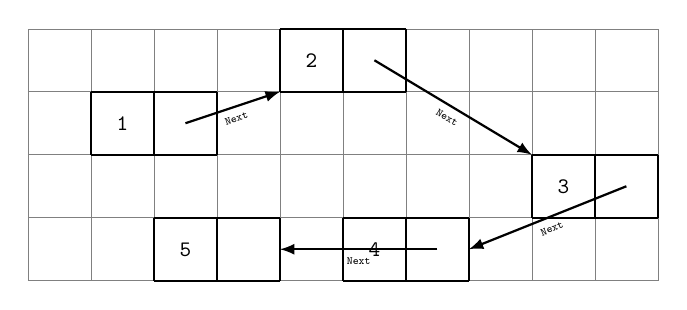
\begin{tikzpicture}[link/.style={thick,-latex},scale=0.8,transform shape]
            \draw[help lines] (0,0) grid (10,4);
            \draw[thick] (1,2) grid ++(2,1);
            \draw[thick] (4,3) grid ++(2,1);
            \draw[thick] (5,0) grid ++(2,1);
            \draw[thick] (2,0) grid ++(2,1);
            \draw[thick] (8,1) grid ++(2,1);

            \draw[link] (2.5,2.5) -- (4,3) node[midway,font=\tiny\ttfamily,sloped,below]{Next};
            \draw[link] (5.5,3.5) -- (8,2) node[midway,font=\tiny\ttfamily,sloped,below]{Next};
            \draw[link] (9.5,1.5) -- (7,0.5) node[midway,font=\tiny\ttfamily,sloped,below]{Next};
            \draw[link] (6.5,0.5) -- (4,0.5) node[midway,font=\tiny\ttfamily,sloped,below]{Next};

            \node[font=\ttfamily] at (1.5,2.5) {1};
            \node[font=\ttfamily] at (4.5,3.5) {2};
            \node[font=\ttfamily] at (8.5,1.5) {3};
            \node[font=\ttfamily] at (5.5,0.5) {4};
            \node[font=\ttfamily] at (2.5,0.5) {5};
        \end{tikzpicture}
    \end{center}
    \vskip4mm
    \code[language=csharp]{LinkedListCreation.cs}
\end{frame}